\documentclass[12pt]{article}
\setlength{\oddsidemargin}{0.0cm}
\setlength{\evensidemargin}{0.0cm}
\setlength{\topmargin}{-2.0cm}
\setlength{\textheight}{22.0cm}
\setlength{\textwidth}{16.0cm}
%\pagestyle{empty}
\usepackage{graphicx}
\usepackage{verbatim}
\begin{document}

\centerline{\Large {\sc Siesta} Exercise: 
MnO, three different magnetic configurations}
\bigskip
{\footnotesize
\begin{verbatim}
SystemName      Manganese Oxide AFM1  # [001] magnetic ordering
SystemLabel            MnO_AF1        # Short name for naming files
%block LatticeVectors
 0.50     0.50      0.0
-0.50     0.50      0.0
 0.0      0.0       1.00
%endblock LatticeVectors
%block AtomicCoordinatesAndAtomicSpecies
 0.00   0.00   0.00  1
 0.00   0.50   0.50  1
 0.0    0.50   0.0   2
 0.0    0.0    0.50  2
%endblock AtomicCoordinatesAndAtomicSpecies
%block DM.InitSpin       # Describe the initial magnetic order (on Mn only)
 1   +
 2   -
%endblock DM.InitSpin

siesta: iscf   Eharris(eV)      E_KS(eV)   FreeEng(eV)   dDmax  Ef(eV)
siesta:    1    -2091.4756    -2068.7533    -2068.7533  0.1524 -0.2680
  (...)
siesta:   15    -2091.1220    -2091.1229    -2091.1229  0.0001 -2.8058

mulliken: Spin UP
Species: Mn
Atom  Qatom  Qorb
               4s      4s      3dxy    3dyz    3dz2    3dxz    3dx2-y2 3dxy
               3dyz    3dz2    3dxz    3dx2-y2 4Ppy    4Ppz    4Ppx
   1  5.588   0.055   0.240   0.990   0.989   0.960   0.989   0.958  -0.010
             -0.016   0.025  -0.016   0.025   0.131   0.137   0.131
   2  0.744  -0.039   0.223   0.034   0.044   0.089   0.044   0.092  -0.006
             -0.007  -0.005  -0.007  -0.004   0.097   0.092   0.097
Species: O
(...)
mulliken: Qtot =       13.000
mulliken: Spin DOWN
Species: Mn
Atom  Qatom  Qorb
               4s      4s      3dxy    3dyz    3dz2    3dxz    3dx2-y2 3dxy
               3dyz    3dz2    3dxz    3dx2-y2 4Ppy    4Ppz    4Ppx
   1  0.744  -0.039   0.223   0.034   0.044   0.090   0.044   0.092  -0.006
             -0.007  -0.005  -0.007  -0.004   0.097   0.092   0.097
   2  5.588   0.055   0.240   0.990   0.989   0.961   0.989   0.958  -0.010
             -0.016   0.025  -0.016   0.025   0.131   0.137   0.131
Species: O
(...)
mulliken: Qtot =       13.000
\end{verbatim}
}
\newpage
\centerline{\Large {\sc Siesta} Exercise: 
MnO, three different magnetic configurations}
\bigskip

{\footnotesize
\begin{verbatim}
SystemName      Manganese Oxide AFM2  # [111] magnetic ordering
SystemLabel            MnO_AF2        # Short name for naming files    
%block LatticeVectors
 1.00     0.50      0.50
 0.50     1.00      0.50
 0.50     0.50      1.00
%endblock LatticeVectors
%block AtomicCoordinatesAndAtomicSpecies
 0.00   0.00   0.00  1
 1.00   1.00   1.00  1
 0.50   0.50   0.50  2
 1.50   1.50   1.50  2
%endblock AtomicCoordinatesAndAtomicSpecies
%block DM.InitSpin       # Describe the initial magnetic order (on Mn only)
 1   +
 2   -
%endblock DM.InitSpin

siesta: iscf   Eharris(eV)      E_KS(eV)   FreeEng(eV)   dDmax  Ef(eV)
siesta:    1    -2091.8778    -2087.1119    -2087.1119  0.9320 -3.3034
(...)
siesta:   14    -2091.2824    -2091.2835    -2091.2835  0.0001 -3.2644

mulliken: Spin UP
Species: Mn
Atom  Qatom  Qorb
               4s      4s      3dxy    3dyz    3dz2    3dxz    3dx2-y2 3dxy
               3dyz    3dz2    3dxz    3dx2-y2 4Ppy    4Ppz    4Ppx
   1  5.512   0.050   0.213   0.991   0.991   0.956   0.991   0.958  -0.016
             -0.016   0.021  -0.016   0.021   0.123   0.123   0.123
   2  0.826  -0.044   0.246   0.040   0.041   0.115   0.041   0.115  -0.007
             -0.007  -0.007  -0.007  -0.007   0.103   0.103   0.103
Species: O
(...)
mulliken: Qtot =       13.000
mulliken: Spin DOWN
Species: Mn
Atom  Qatom  Qorb
               4s      4s      3dxy    3dyz    3dz2    3dxz    3dx2-y2 3dxy
               3dyz    3dz2    3dxz    3dx2-y2 4Ppy    4Ppz    4Ppx
   1  0.826  -0.044   0.246   0.040   0.041   0.115   0.041   0.115  -0.007
             -0.007  -0.007  -0.007  -0.007   0.103   0.103   0.103
   2  5.512   0.050   0.213   0.991   0.991   0.956   0.991   0.958  -0.016
             -0.016   0.021  -0.016   0.021   0.123   0.123   0.123
Species: O
(...)
mulliken: Qtot =       13.000
\end{verbatim}
}
\newpage
\thispagestyle{empty}
\normalsize
\centerline{\Large {\sc Siesta} Exercise: 
MnO, three different magnetic configurations}
\bigskip

\setlength{\unitlength}{1.0cm}
\begin{picture}(0,0)
\put(-1.0,-15.0){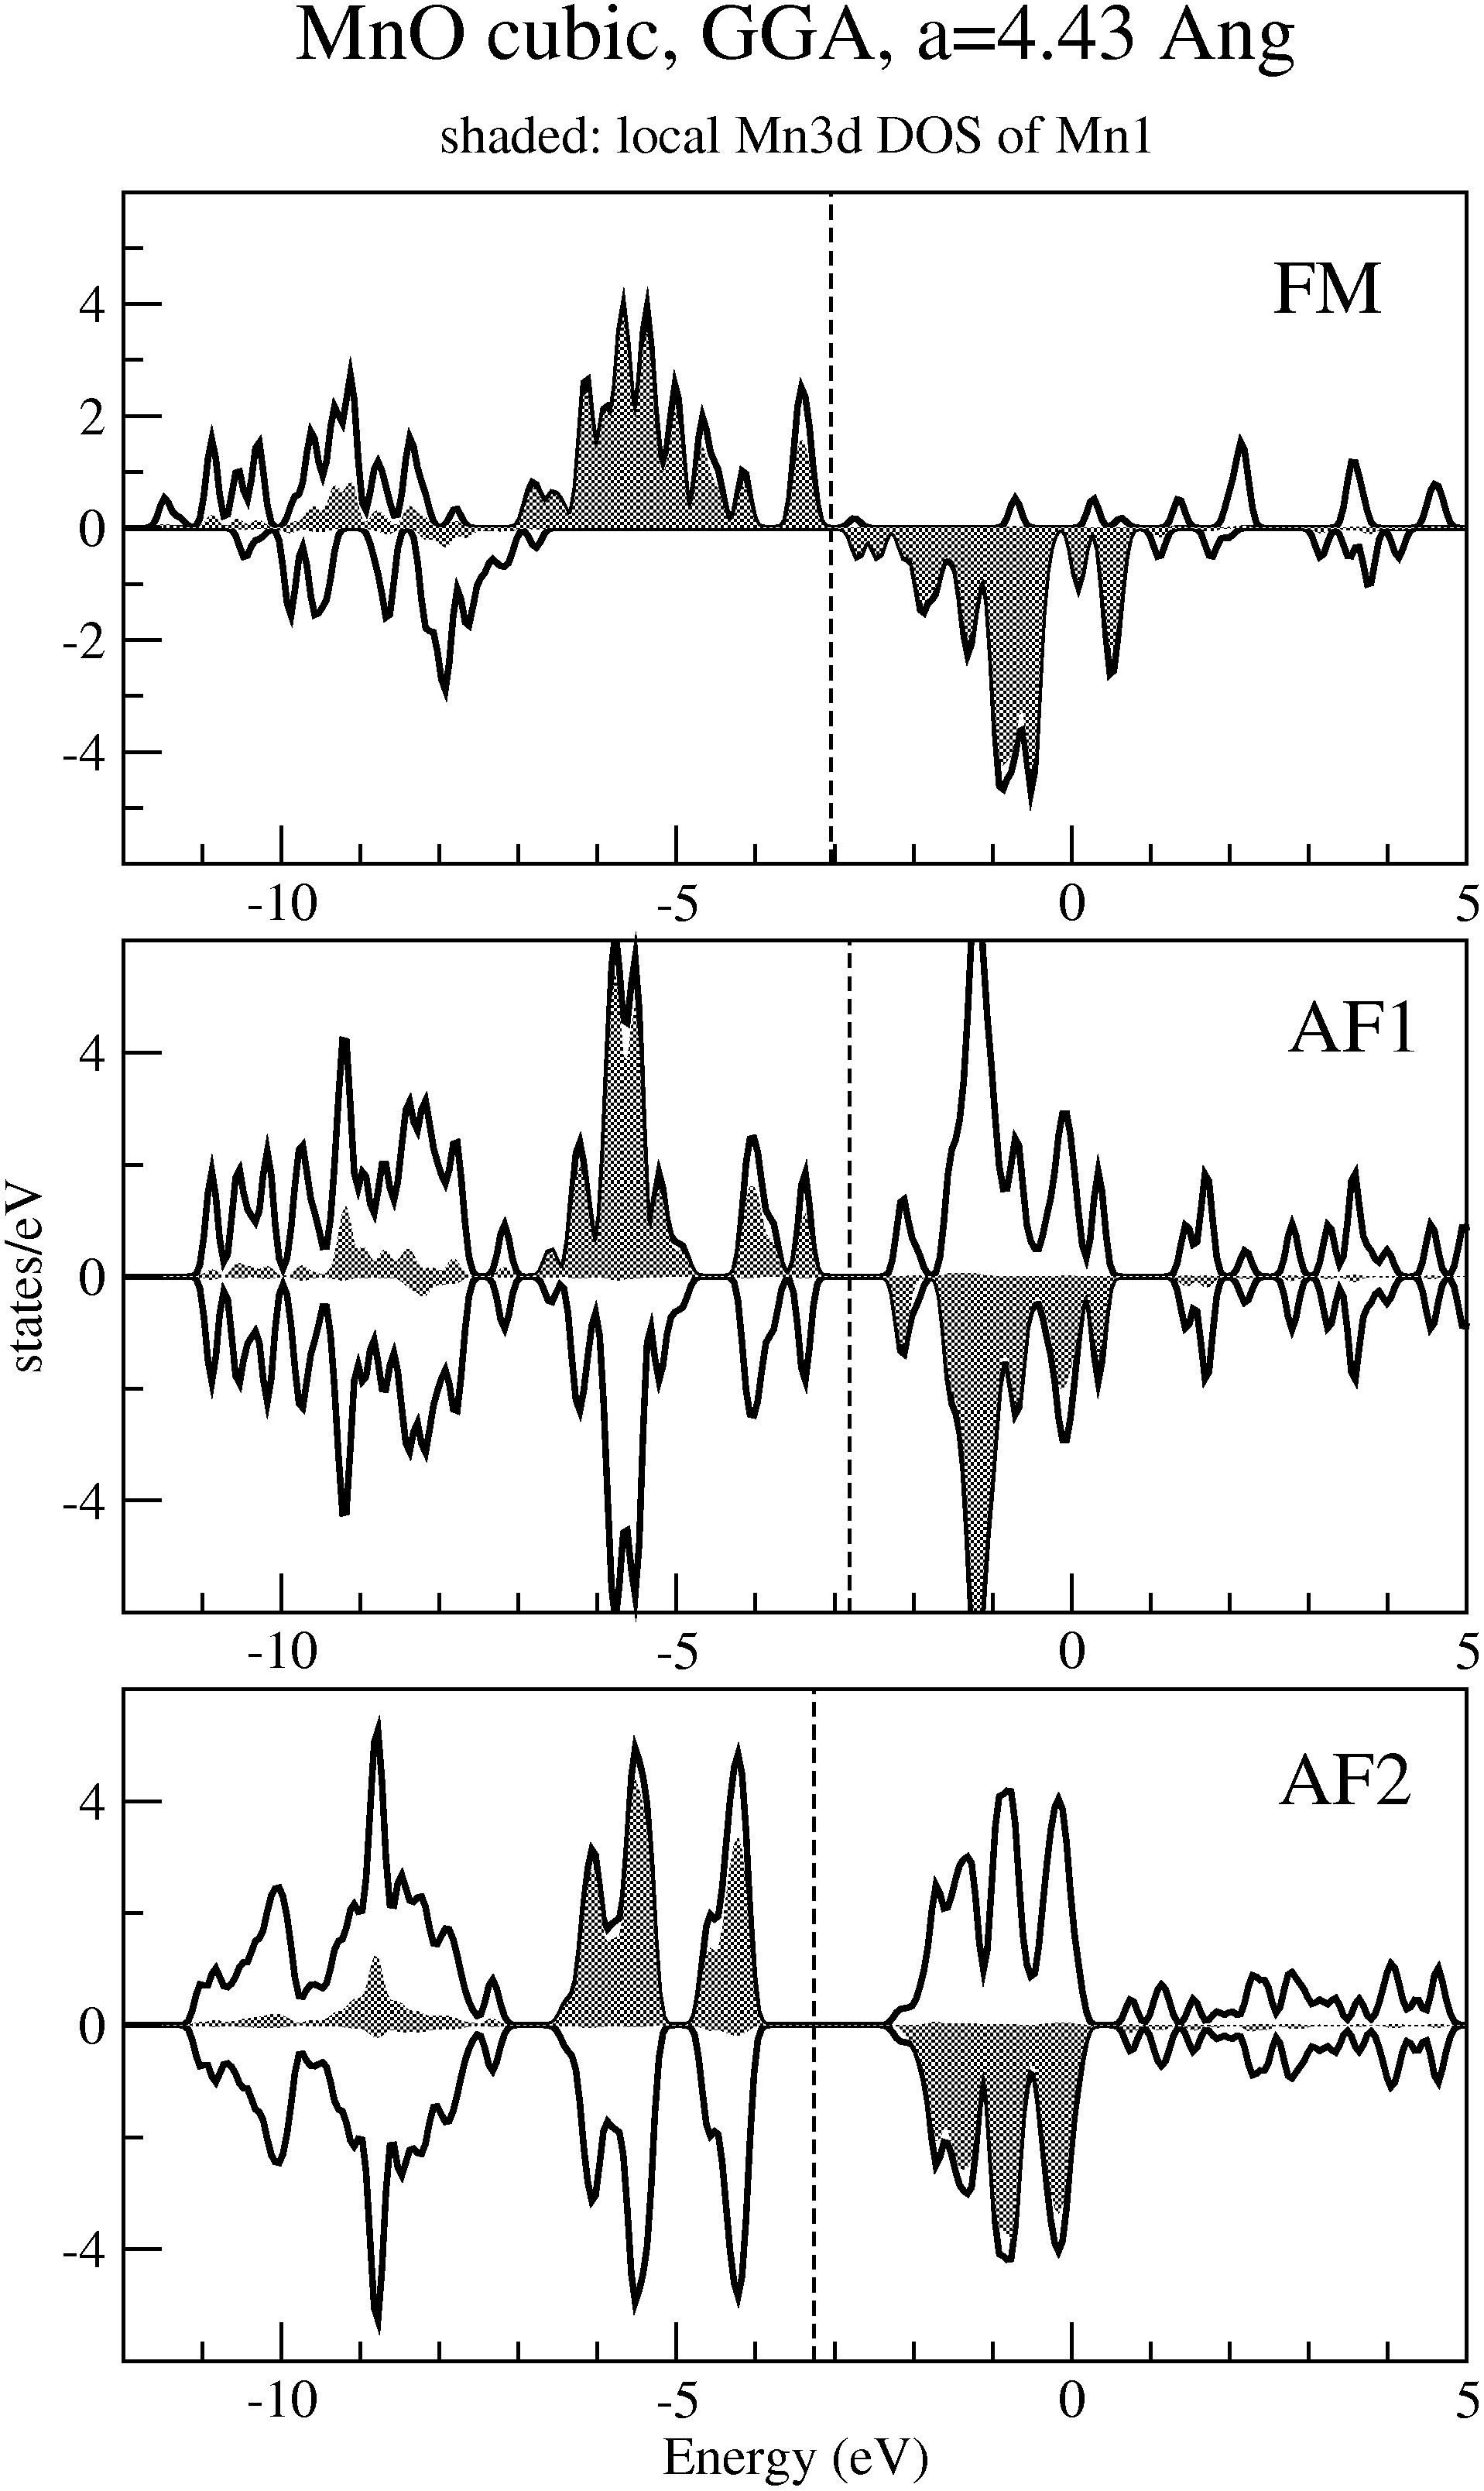
\includegraphics[width=9.0cm]{DOS_figure.png}}
\put(9.0,-2.0){\parbox[t]{7.0cm}{
Left figure:\\*[1mm]
Spin-resolved \\local (at Mn site) and total (per unit cell)
densities of states.
}}
\put(9.5,-9.5){\parbox[t]{7.0cm}{
Bottom figure:\\*[1mm]
Spatial magnetic density (levels $\pm$0.2) shown by different colours.
\\*[2mm]
Think why the surfaces are so spherical around each Mn atom.
\\*[1mm]
Try to identify $t_{2g}$ and $e_g$ states in the occupied part
of the Mn$3d$ DOS of AF2 structure, calculate and visualize LDOS
separately for these two groups of states. 
}}

\put(0.0,-20.0){
\put(-2.5, -2.1){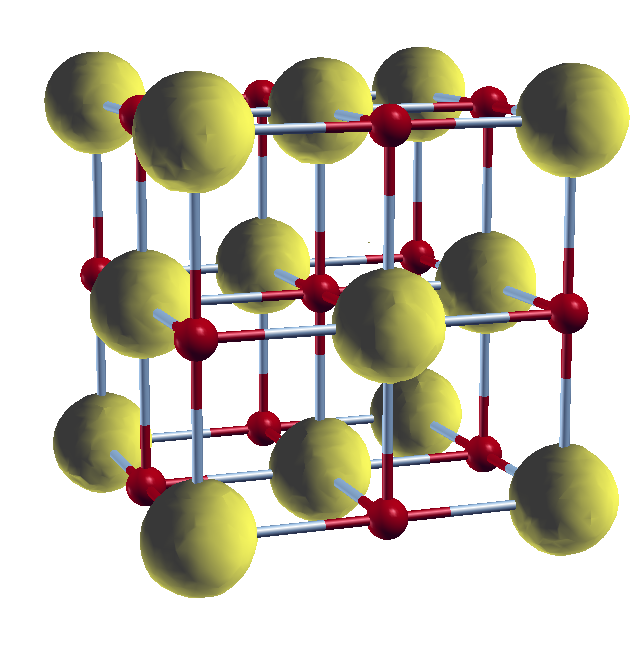
\includegraphics[width=6.6cm]{MnO_FM.png}}
\put( 0.8,-2.2){\Large FM}
\put(4.5, -2.0){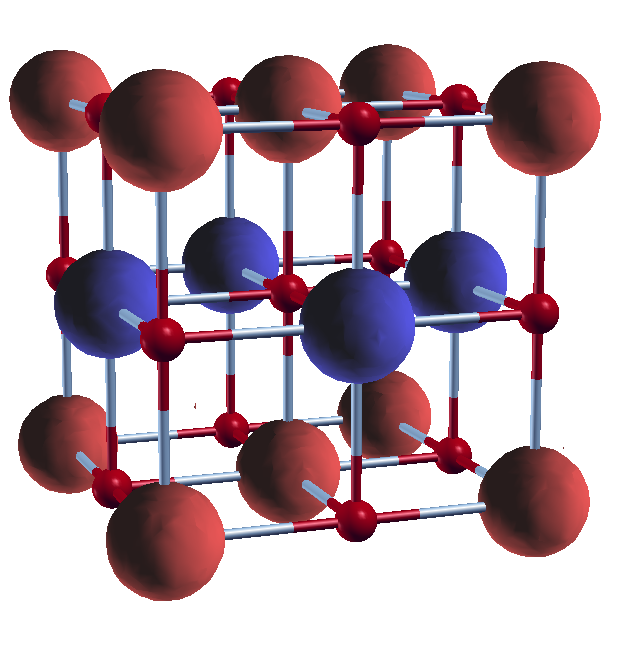
\includegraphics[width=6.5cm]{MnO_AF1.png}}
\put( 7.4,-2.2){\Large AF1}
\put(11.0,-2.0){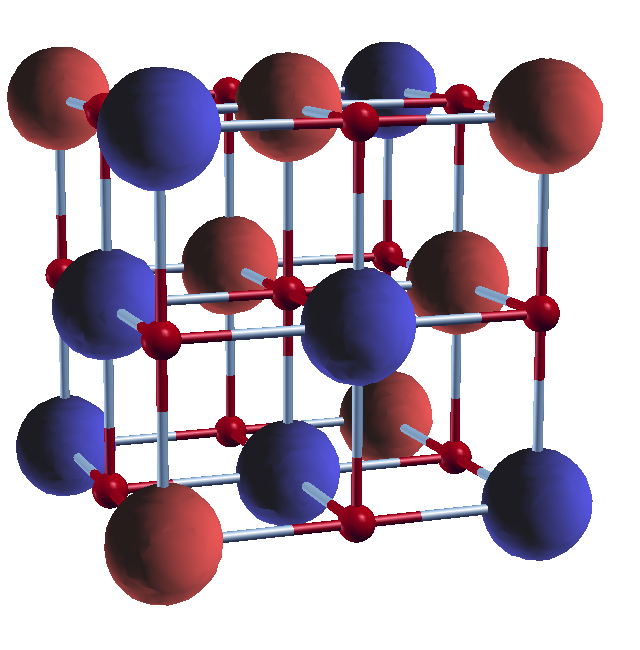
\includegraphics[width=6.5cm]{MnO_AF2.png}}
\put(14.0,-2.2){\Large AF2}
}
\end{picture}
\end{document}
